\chapter{Pattern recognition}
\label{ch:pattern-recognition}
\minitoc

The diagram below is due to David Marr:
\begin{figure}[H]
\centering
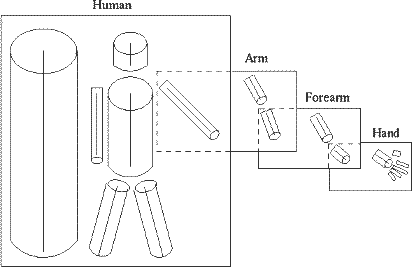
\includegraphics[scale=0.7, viewport=0 0 414 269]{Marr3DModel.PNG}
\end{figure}

A highly simplified example of pattern recognition is the visual recognition of a human body by a Prolog rule such as\footnote{
Note that these concepts refer to \textit{visual features} rather than ideas  (The abstract concept of a human can be recognized via a larger set of rules that includes the visual rules).  The visual features should also be related to each other by some spatial predicates, but we ignore them here.  The details of visual recognition is explained in \S\ref{ch:vision}.
}:\\
\hspace*{1cm} \code{human :- head, torso, arm1, arm2, leg1, leg2.}\\
and each body part can be further recognized by its components such as:\\
\hspace*{1cm} \code{arm1 :- upper-arm, forearm, hand, fingers.}

In general the mechanism for pattern recognition is \textbf{forward-chaining} because we start with the premises (sensory input) and we do not know the desired conclusions in advance.

\section{The theory-based theory}

Concept formation (or ``categorization'' in the cognitive science literature, \citep*{Murphy2002}, \citep*{Cohen2005}, \citep*{Margolis1999}, \citep*{Lakoff1987}) is the task of using machine learning to learn common-sense concepts (\citep*{Nakamura1993}, \citep*{Wrobel1994}).  \citep*{Wrobel1994} has summarized the following properties of human concepts:
\begin{compactenum-}
\item concepts often have non-necessary features
\item disjunctive concepts (there may not be any features that are shared by all members of a concept)
\item relational information (seems to require first-order logic to represent)
\item some features are themselves concepts
\item typicality (people can often rank examples according to typicality, eg the most typical fruit is orange)
\item basic levels (people are more adapt at categorization at certain basic levels, eg naming an object ``chair'' rather than ``office chair'' or ``a piece of furniture'')
\item superordinate distance (eg ``chicken'' is rated more similar to ``animal'' than to ``bird'')
\item unclear cases (eg ``is tomato a fruit?'')
\item context-dependent effects
\item goal-dependent effects
\end{compactenum-}

There are two major theories of categorization:  In the \textbf{Classical view} a concept is defined by a set of defining features which are individually necessary and sufficient.  This view has very few adherents now.  The other major theory is the \textbf{Exemplar view}, which classifies instances based on their similarity (eg a distance metric) to a set of existing exemplars.

In my opinion, also shared by \citep*{Murphy1985} and \citep*{Wrobel1994}, the most satisfactory solution (aka the \textbf{theory-based theory}) is to view categorization as an \textit{inference} process, where concept formation means constructing \textit{explanations} of why certain objects belong to a concept.

\section{Similarity}
\label{sec:similarity}

Similarity is an essential component of commonsense reasoning.  For example, if we are told that "the whale is like a fish except that it is a mammal" we could draw the conclusion that the whale can swim (because fishes usually can swim) \footnote{But we would not conclude that the whale lays eggs because mammals don't lay eggs and we know that the whale \emph{is} a mammal, but it is only similar to a fish, and "is" is stronger than "similar to".}.  The similarity measure may also help in associative recall (\S\ref{sec:associative-memory}).

\subsection{From equality to similarity}

 Similarity ($\approx$) can be viewed as a generalization of the equality relation ($=$) with fuzzy-probabilistic truth.  For example we can write\\
\tab $\mbox{whale} \approx \mbox{fish}$.

Equality ($=$) can be defined via \textbf{Leibniz's axiom of extensionality} -- which states that 2 functions are identical if their extensions are the same.  In higher-order logic it can be expressed as:
\begin{equation}
\forall x [f x = g x]  \Leftrightarrow f = g
\label{eqn:Leibniz-extensionality}
\end{equation}
with types $x : \beta$ and $f, g : \beta \rightarrow \alpha $.  This definition of $=$ is given by Church's type theory in 1940.  

$\approx$ can be regarded as the probabilistic version of $=$.  We can simply replace the $\forall$ quantification in (\ref{eqn:Leibniz-extensionality}) with the probabilistic quantification $\#$ (\S\ref{sec:probabilistic-quantifier}), as in:
\begin{equation}
\# x [f x = g x] \Leftrightarrow f \approx g.
\label{eqn:probabilistic-extensionality}
\end{equation}
% And because we can use fuzzy truth values, the $=$ on the LHS can also be replaced with a fuzzy version and we might denote it as $\approx$ as well:
% \begin{equation}
% \# x [f x \approx g x] \Leftrightarrow f \approx g.
% \label{eqn:probabilistic-extensionality}
% \end{equation}

% And the probabilistic form is:
% \begin{equation}
% \# z [z x \approx z y]  \Leftrightarrow x \approx y.
% \end{equation}

\subsection{Leibniz extensionality and intensionality}

Our strategy is this:  first we will formulate the most general form of semantic similarity, which we expect to be computationally intractable, then we try to approximate it.

Leibniz extensionality (\ref{eqn:Leibniz-extensionality}) defines equality for functions or predicates, but not for individual objects.  For the latter purpose we have to invert extensionality to \textit{intensionality} as follows:
\begin{eqnarray}
\mbox{(extensionality)}    & \forall Z. [x Z  = y Z] & \Leftrightarrow x = y \label{eqn:extensionality} \\
\mbox{(intensionality)}     & \forall Z. [Z x  = Z y] & \Leftrightarrow x = y \label{eqn:intensionality}
\end{eqnarray}
where I have renamed variables to stress the symmetry.  The second axiom says that 2 entities are the same if every property of one is also a property of the other.

An example of intensionality (which may be more common than extensionality) is:

\tab \tab \tab
\begin{tabular}{l|l}
has-fins(whale)           & has-fins(fish)\\
lives-in(whale, water) & lives-in(fish, water)\\
vertebrate(whale)      & vertebrate(fish)\\
\hline
\multicolumn{2}{c}{$\therefore \;$ whale $\approx$ fish}
\end{tabular}

Notice that $Z$ is a higher-order variable in (\ref{eqn:intensionality}), which can be \textit{instantiated} as n-ary predicates with other arguments, eg:
 $$Z(x) = \mbox{lives-in}(x, \mbox{water})$$
so together with extensionality this offers a very powerful way to express all possible forms of similarities, and may be regarded as a logic-based, alternative formulation of Ulf Grenander's Pattern Theory \citep*{Grenander2007}.  But (\ref{eqn:extensionality}) and (\ref{eqn:intensionality}) require higher-order unification which is highly intractable.

In our new ``combinatory'' logic (\S\ref{}), there is no need to deal with structured terms with functions, since all terms are built up solely via composition.  Thus we can combine extensionality with intensionality into:
\begin{equation}
\mbox{(similarity)} \quad \forall C. \; C[ x ] , C[ y ] \Leftrightarrow  x \approx y 
\label{eqn:similarity}
\end{equation}
where $C$ denotes a context, ie, $C[x] = C_1 x \, C_2 = c_1 c_2 ... x \, c_{i+1} c_{i+2} ... $, ie, a term with a hole in it.  (\ref{eqn:similarity}) is the most general form of similarity.  This kind of pattern-matching is exactly the kind handled by \textbf{unification} (\S\ref{sec:unification}), that means we know, at least in theory, the inference algorithm to calculate similarities, though it would be inefficient.  Now the question is to approximate it.

% \{ To-do:  I need to develop the above theory further.  Milner's Context Lemma in domain theory (see eg \citep*{Streicher2006}) seems to have some semblance to what we're doing here.  Milner's Lemma states the equivalence of 2 orderings, $<_{\sigma}$ and $\sqsubset$.  They are defined by:
% \begin{eqnarray}
% M \sqsubset N  \quad  &\mbox{iff}& \quad \forall z \in \setN. \; M \Downarrow z \Rightarrow N \Downarrow z \\
% M <_{\sigma} N \quad  &\mbox{iff}& \quad \forall Z \in \mbox{programs.} \; Z(M) \sqsubset Z(N)
% \end{eqnarray}
% where $M \Downarrow z$ means $M$ evaluates to $z$.  The situation kind of resembles Leibniz's definition and its inverted form.
% \}

\subsection{Distance metric}

Our goal is to find an algorithm that calculates the distance $d(T_1, T_2)$ between 2 arbitrary logic terms.  Using the sum-of-products form, first we try to define the distance $d(P_1, P_2)$ between 2 products.  One way to do this may be to assign to each atomic concept $c$ a matrix $m_c$, so they form a basis set in a matrix space.  Then a product $P = \prod c_i$ would have a matrix value $M = \prod m_i$.  Then we find the distance $d(P_1, P_2)$ by calculating $d(M_1, M_2)$ as the distance between 2 matrices, which can be defined via the inner product $\langle x,y \rangle$ \footnote{The inner product between 2 matrices can be defined as $\langle A, B \rangle  := tr \; A^T B$ for real matrices and $tr \; A^*B$ for complex matrices, where $tr$ is the trace and $A^*$ is the adjoint matrix which is equal to the conjugate transpose (alias Hermitian transpose, $A^H$) of $A$, ie, with entries $\overline{a_{ji}}$.  So $ d(M_1, M_2) =  \sqrt{tr \; M_1 ^* M_2} $.}:
$$ d(M_1, M_2) := || M_1 - M_2 || := \sqrt{\langle M_1 - M_2, M_1 - M_2 \rangle} .$$

Next, the distance between 2 sums $\sum P^1_i$ and $\sum P^2_j$ can be defined as:
\begin{equation}
{\displaystyle \sum_i {\displaystyle \min_j } \; d(P^1_i, P^2_j) }
\label{eqn:sum-distance}
\end{equation}
or in other words, the minimal sum of distances between pairs of products ($P^1_i$'s and $P^2_j$'s).

Then we can use a learning algorithm to tweak the values of the basis matrixes $m_c$.  For example, \english{cat} is similar to \english{dog} so we can move the matrices $m_{cat}$ and $m_{dog}$ closer to each other.  Conversely, if 2 products are known to be semantically close, we can gradually \textbf{propagate} their numerical similarity back to their constituent atomic concepts.

\question{Is it always possible to maintain the distances in such a matrix space, consistent with our notion of similarity?  What would be some counter-examples? }

\subsubsection{Formulas with variables}

For example: $a \, X \, b \, Y \, c$.  If a variable $X$ can take any matrix value, the product map end up in any position in the matrix space.  But, we may be able to establish some (hard or soft) constraints over $X$, such that the resulting product would be confined in certain regions.  It seems that a formula with variables would be some sort of ``hyperplane'' in the matrix space.  We can still define the distance between a hyperplane and other matrices.

\subsection{Examples}

\textbf{(A)} From:\\
\tab dog $\approx$ cat, \\
using the backward direction of (\ref{eqn:similarity}) we can deduce: \\
\tab let sleeping dogs lie $\approx$ let sleeping cats lie \\
but the result is incorrect and un-idiomatic.  \question{Does it break our matrix-based method? }

\textbf{(B)} The following idioms are similar in semantics but dissimilar in syntax:
\begin{figure}[H]
\centering
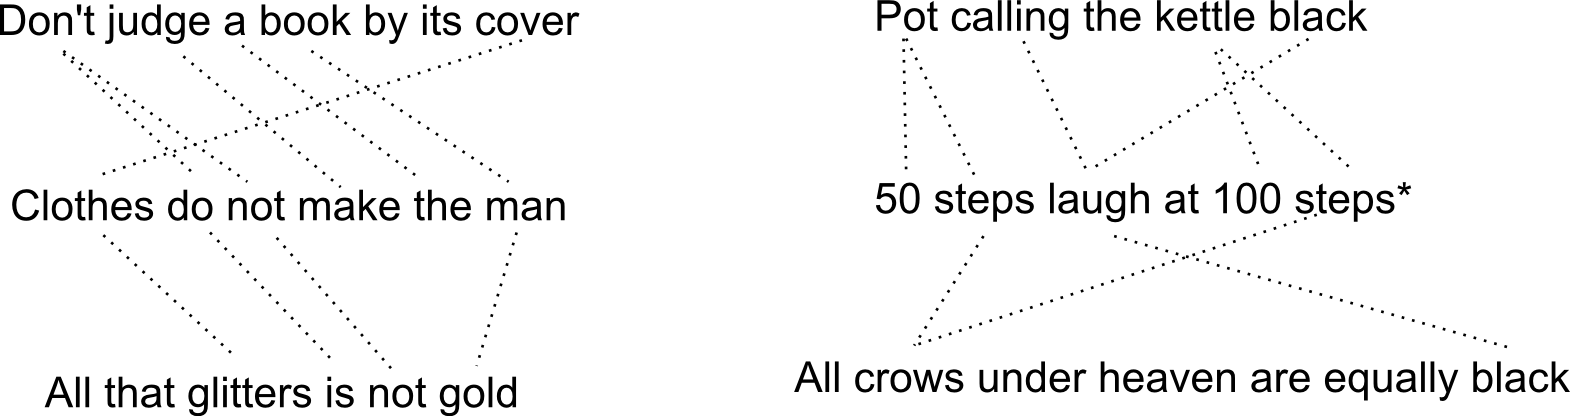
\includegraphics[scale=0.8]{similar-idioms.png}
\end{figure}
\vspace{-1em}
\renewcommand{\thefootnote}{\fnsymbol{footnote}}
\footnotetext[1]{Chinese idiom: \english{Those who retreated 50 steps laugh at those who retreated 100 steps}.}
\renewcommand{\thefootnote}{\arabic{footnote}}
but there are some weak / fuzzy correspondence between their words.  \question{Does it break our matrix-based method?  If not, how can we back-propagate the similarities to their atomic concepts? }

\textbf{(C)} We'd be interested in measuring similarities between entities with certain structures.  This has been considered, eg in \citep*{Schmid2003}, chapters 10-12, in an ILP setting.  A famous example is the similarity between the solar system and the atom:  the important point is that both systems have bodies revolving around a central body, but it does not matter what their size, mass, and temperature, etc, are.

\{ The text that follows is outdated... \}
\underconst

What we seek is a correspondence between 2 structured entities, and to quantitatively measure the strength of such a correspondence.  Perhaps we can count the number of relations common to both entities.

\textbf{(D)} ``Marmite is similar to Vegemite''\\
\hspace*{1cm} \begin{tabular}{l|l}
salty(marmite)                   & salty(vegemite)\\
dark-brown(marmite)              & dark-brown(vegemite)\\
yeast-extract(marmite)           & yeast-extract(vegemite)\\
rich-in(marmite, vitamin B)      & rich-in(vegemite, vitamin B)\\
sub-string(name(marmite),"mite") & sub-string(name(vegemite),"mite")\\
popular-in(england)              & popular-in(australia)
\end{tabular}

So I propose that the similarity between 2 objects can be calculated by considering all predicates that apply to both objects and obtaining the ratio between the number of identical and different predicates:
\begin{equation}
\mbox{similarity } \; \psi = \frac{N^{=}}{N^{=} + N^{\neq}}
\end{equation}

\{ TO-DO:  If the predicates have complex structure, we need to (recursively) compare the other arguments, and if the latter are different, adjust for their differences. \}

The above calculation can also be weighted by \textbf{information utility}, yielding the \textbf{subjective similarity} measure.

NOTE:  (E) is a bad example and should be replaced by something else.\\
(E) ``Lincoln is similar to Kennedy''
\footnote{In this example I have used my own knowledge representation scheme Geniform.  The example is based on a series of uncanny coincidences between the Lincoln and Kennedy assassinations that are often cited in trivia books.}
\\
\hspace*{1cm} \begin{tabular}{l|l}
elected-to-congress(lincoln, 1846)        & elected-to-congress(kennedy, 1946)\\
elected-president(lincoln, 1860)          & elected-president(kennedy, 1960)\\
succeeded-by(lincoln, vice-president$_1$) & succeeded-by(kennedy, vice-president$_2$)\\
\hspace*{1cm} name(vice-president$_1$, "johnson") &
\hspace*{1cm} name(vice-president$_2$, "johnson")\\
\hspace*{1cm} born(vice-president$_1$, 1808) &
\hspace*{1cm} born(vice-president$_2$, 1908)\\
assassinated$_1$(lincoln, friday)         & assassinated$_2$(kennedy, friday)\\
in(assassinated$_1$, theater)             & in(assassinated$_2$, car)\\
name(theater, "ford")                     & made(car, "ford")\\
with$_1$(wife(lincoln), lincoln)          & with$_2$(wife(kennedy), kennedy)\\
\hspace*{1cm} during(with$_1$, assassination$_1$) &
\hspace*{1cm} during(with$_2$, assassination$_2$)\\
\end{tabular}

Additionally:\\
\hspace*{1cm} name(car, "Lincoln")\\
\hspace*{1cm} has(kennedy, secretary), name(secretary, "Lincoln")

The additional facts do not increase the similarity, but they do make the 2 cases seem more ``connected''.

\underconst

(C) Some quantitative examples:\\
\hspace*{1cm} \begin{tabular}{|l|l|l|}
\hline
\textbf{the thing} & \textbf{approximated as} & \textbf{reason}\\
\hline
orange T-shirt     & red T-shirt      & proximity in color space\\
7 people           & several people   & $\catZ$\\
6'5 tall           & very tall        & $\catZ$\\
(John lies on several occasions) & John often lies & $\catP$\\
Stewart Shapiro    & Stuart Shapiro   & string edit distance\\
\hline
\end{tabular}

These examples can be represented and approximated by $\mathcal{P/Z}$ values (eg with fuzzy pattern recognition).

%orange(t-shirt) -> red(t-shirt)
%7*people -> several*people
%height(john,6.5) -> tall(john)
%(multiple facts) -> lies1(john), often(lies1)
%"Stewart Shapiro" -> "Stuart Shapiro"

(D) Some qualitative examples:\\
\hspace*{1cm} John is humorous $\approx$ John is witty\\
\hspace*{1cm} junk food, smoking and drinking $\approx$ unhealthy lifestyle\\
\hspace*{1cm} theft $\approx$ burglary\\
\hspace*{1cm} (complex scene) $\approx$ a fighting in a bar

